%*****************************************
\chapter{Evaluation}\label{ch:evaluation}
%*****************************************

All tests were carried out on a laptop running Linux Mint 10.0, using a 1.46 Ghz Intel Pentium dual core CPU with 1 GiB of RAM.

For comparison, Firefox 4.0's minumum requirements include a single core 1.4 Ghz CPU with 512Mb of RAM. The average broadband speed in the UK is around 10 Mbps \url{http://www.netindex.com/download/2,4/United-Kingdom/}. 

\section{Conduit image performance}

For each conduit image implementation we consider the theoretical channel capacity. When used in conjunction with a forward error correction scheme we can also consider the actual per-image useful data rate and final output error probability.

The per-image channel capacity of a conduit image implementation is the function of the amount of information the implementation can store in a single image (equivalently the symbol size) and the signal to noise ratio. We model the compression/decompression process as a binary symmetric channel and calculate the channel capacity for arbitrarily small error probability, using a measured bit error rate as an estimate for the bit error probability.

We analyse each implementation when used with a forward error correction scheme, presenting the resultant per-image transfer rate and output decoder error probability.

\subsection{Method}

The relevant library components are loaded into a test C++ file. A standalone conduit image instance is created and a random byte vector generated and encoded. The result is saved to disk as a JPEG at a given quality factor, reloaded and the data decoded. We log the Hamming distance between the input and output data and the time taken to perform each encode and decode. This process is repeated until the cumulative amount of data processed exceeds 1 GiB. The test was repeated for each of the three conduit image classes and also for quality factors 80-90. Timings were recorded using CPU time and excluded time spent generating random numbers, performing compression or writing out to/reading from disk.

\begin{table}[tbp]
  \begin{center}
        \begin{tabular}{l l l l l}
        \textbf{Method} &\textbf{Bits per} &\textbf{Test set size} & \textbf{Test set size} &\textbf{Possible unique} \\ 
            &\textbf{block} &\textbf{(images)} &\textbf{(blocks)} &\textbf{blocks} \\ [0.1ex] \hline \\ [-1.5ex]
        Scaled3	&192	&5,523	&44,736,300	& $6.28 \times 10^{57}$ \\
        Scaled4	&256	&4,142	&33,550,200	& $1.16 \times 10^{77}$ \\
        Haar	&24	&44,186	&357,906,600	& $1.68 \times 10^{7}$ \\
        \end{tabular}
        \caption{Tabulated details of the testing process. \textasciitilde 1 GiB of data was used for every test run.}
        \label{tab:img-test}
    \end{center}
\end{table}


Table \ref{tab:img-test} summerises the number of useful bits each method can store in a single 64 x 8 bit greyscale JPEG luminance block along with the effective sample size (number of images/blocks processed during the test) and population size (total number of possible unique blocks) we are sampling from. Due to the size of the samples the standard error is negligable, even before applying finite population correction where appropriate (see appendix XXX for details).

The results in section XXX were obtained by repeating the first test with an additional encode and decode stage at which point error correction codes were added.

\subsection{Theoretical capacity}

We model each conduit image as a binary symmetric channel: we know the encoding/decoding process does not result in bit erasures; we make the assumption that the probability of error $p_e$ is independant and equal for each bit. Given the large sample sizes (see appendix XXX) we can assume that the measured bit error rate is a reasonable estimate of the actual bit error probability.

The formula used to calculate the capacity is obtained by taking the typical capacity calculation for a binary symmetric channel and multiplying by the number of bits available per image $A$, to obtain:

\begin{equation}
    C = A \cdot (1 + H(p_e))
\end{equation}

Where $H(x)$ is the binary entropy function. This provides the capacity in units of information per symbol - in this case bits per image. Figure \ref{graph:capacity} compares the calculated capacity for each of the three conduit images implementations. At quality factor 85, which most closely matches the profile of the Facebook JPEG compression proccess, we see both scaling methods performing approximately the same with capacities of over 180 KiB per image.

\begin{figure}[tbp]
  \begin{center}
\begin{tikzpicture}
    \begin{axis}[grid=major,xlabel=JPEG Quality Factor,ylabel=BER (\%), xmin=80, xmax=90,
    height=9cm,width=11cm,legend style={legend pos=outer north east}]
    
    \addplot
        table[x=QF,y=Sc3] {gfx/error_rate.data};
    
    \addplot
        table[x=QF,y=Sc4] {gfx/error_rate.data};
        
    \addplot
        table[x=QF,y=Haar] {gfx/error_rate.data};
        
    \legend{Scaled3,Scaled4,Haar}
    
    \end{axis}
\end{tikzpicture}
    \caption{Bit error rate for varying quality factors.}
    \label{graph:ber}
  \end{center}
\end{figure}

\begin{figure}[tbp]
  \begin{center}
\begin{tikzpicture}
    \begin{axis}[grid=major,xlabel=JPEG Quality Factor,ylabel=Capacity (KiB/image), xmin=80, xmax=90,
    height=9cm,width=11cm,legend style={legend pos=outer north east}]
    
    \addplot
        table[x=QF,y=Sc3] {gfx/encoding_time.data};
    
    \addplot
        table[x=QF,y=Sc4] {gfx/encoding_time.data};
        
    \addplot
        table[x=QF,y=Haar] {gfx/encoding_time.data};
        
    \legend{Scaled3,Scaled4,Haar}
    
    \end{axis}
\end{tikzpicture}
    \caption{Per-image channel capacity (measured in KiB/image) for varying quality factors.}
    \label{graph:capacity}
  \end{center}
\end{figure}

\subsection{Reed Solomon error correction}

Given the bit error probability $p$ we can obtain the symbol error probability $p_s$:

\begin{equation}
    p_s = 1 - (1-p)^m
\end{equation}

where $m$ is the number of bits per symbol. In general, for a Reed Solomon code with symbol error probability $p_s$ the decoded symbol error probability $p_s'$ is given by:

\begin{equation}
    p_s' = \frac{1}{2^m -1} \sum^{2^m - 1}_{i = t+1} i {{2^m - 1}\choose{i}} {p_s}^i (1-{p_s})^{2^m - 1 - i}
\end{equation}

where $t$ is the maximum number symbol errors we can correct \cite{rsfec-decode}. Both the concrete error correction classes in the Encrypted Facebook library are based on Reed Solomon error correction. The (15,9) code can correct up to $t=3$ symbol errors and has a 4-bit symbol size. The (255,223) code can correct up to $t=16$ symbol errors and has a 8-bit symbol size.

The decoded symbol error probability $p_s'$ we may consider as an upper bound for the decoded bit error probability. Figure \ref{tab:fec} tabulates error probabilities for each FEC used based on the measured bit error rate as an estimate, assuming a JPEG quality factor of 85.

\begin{table}[h]
  \begin{center}
        \begin{tabular}{l l l l l l}
            
            \textbf{Method} & \textbf{FEC} & \textbf{$p$} & \textbf{$p_s$} & \textbf{$p_s'$} & \textbf{Capacity (KiB)} \\ [0.1ex] \hline \\ [-1.5ex]

            Haar & (15,9) & $4.20 \times 10^{-3}$ & $1.67 \times 10^{-2}$ & $2.47 \times 10^{-5}$ & 14.2 \\
            Haar &  (255,223) & $4.20 \times 10^{-3}$ & $3.31 \times 10^{-2}$ & $3.73 \times 10^{-4}$ & 20.8 \\
            Scaled3 & (15,9) & $8.30 \times 10^{-4}$ & $3.32 \times 10^{-3}$ & $4.28 \times 10^{-8}
$ & 113.9 \\
            Scaled3 & (255,223) & $8.30 \times 10^{-4}$ & $6.62 \times 10^{-3}$ & $1.81 \times 10^{-13}
$ & 166.0 \\
            Scaled4 & (15,9) & $4.49 \times 10^{-2}$ & $1.68 \times 10^{-1}$ & $7.14 \times 10^{-1}$ & 151.9 \\
            Scaled4 & (255,223) & $4.49 \times 10^{-2}$ & $3.08 \times 10^{-1}$ & $3.08
 \times 10^{-1}$ & 221.4 \\
            
        \end{tabular}
        \caption{Table of stuff.}
        \label{tab:fec}
    \end{center}
\end{table}

Haar with 15,9: 0.000332178
Haar with 255,223: 0.000372675
Scaled3 with 15,9: $6.50148 \times 10^-7$, equiv, : $1.3 \times 10^-6$
Scaled3 with 255,223: $1.68634 \times 10^-13$


Should on in a million Gb, or one in a trillion images. This NASA document url{http://ipnpr.jpl.nasa.gov/progress\_report/42-84/84F.PDF} shows what they used for the Voyager space probe. Also this approaches hard drive read/write error rates.

\section{Cognitive walkthrough}

\cite{cogwalk}

Use Upsampled3 since we've shown its the best

For one user, X:

\begin{itemize}
    \item Create a crypto identity.
    \item Migrate profile information.
\end{itemize}

Now create 15 more users, friends of user X. (group A). Also have one user who is not a recipient (group B). And one more user who doesn't have application at all (group C). Repeat encryption headers 28 times so we simulate group of size 405. Also repeat entries in UI controls.

\begin{itemize}
    \item Public key management - add keys of group A to user X.
    \item Text submission - from X to group A.
    \item Image submission - from X to group A.
    \item Text and image retrieval - for user X.
    \item Text and image retrieval - for one member of group A.
    \item Text and image retrieval - for group B.
    \item Text and image retrieval - for group C.
\end{itemize}

\section{Profiling submission and retrieval}

To measure mean encode/decode and upload/download times for a single object automated tests were ran programmatically from the extension, with each submission and retrieval round being allowed to complete before beginning the next.

To obtain results which tested real-world performance and included the full set of DOM tree navigation/insertion operations and browser pageload times additional retrieval tests were performed. Pages containing multiple items of encrypted content were loaded, triggering asynchronous retrieval and deocoding. For comparison these tests were repeated with the extension disabled.

\subsection{Method}

All encryption was performed with a simulated group size of 405 as detailed in section XXX. Test images were duplicate copies of a (approximately) 50 KiB JPEG image (see section XXX). Test messages were randomly generated strings of mixed-case letter and numeral characters. With the exception of the last test where strings were limited by the 420 character status update length limit, messages were 10,000 characters in length - the limit for private messages.

A modified version of the Chromebug Firefox extension was used to record all results.

\subsubsection{Synchronous submission \& retrieval}

For textual content, 1000 messages were generated. The note submission function was then called with each message using a 60 second delay in between each run - leaving enough time for one submission and retrieval round to complete before beginning another. The tags required to retrieve these notes are saved and the time spent in each submission phase profiled. When the HTTP request for sumbmission completes, retrieval is triggered and the download and decoding time logged. The same test was repeated using a set of 1000 images.

\subsubsection{Asynchronous retrieval}

Sample newsfeeds were generated with 15 status update entries, as this is the number of newsfeed entries Facebook first loads \footnote{More are loaded dynamically when the user scrolls to the bottom of the page.}. Status update messages were random ASCII text 420 characters in length, the maximum permitted. One newsfeed contained plaintext entries and the other contained encrypted entries generated through the plugin. The pages were loaded repeatedly 1000 times and the loading and retrieval times logged. In between each load both the browser cache and extension cache were deleted. The entire process was then repeated for a newsfeed containing 15 image entries, once again random images of size 50 KiB, instead of status messages.

\subsection{Results}


\begin{figure}[tbp]
    \begin{center}
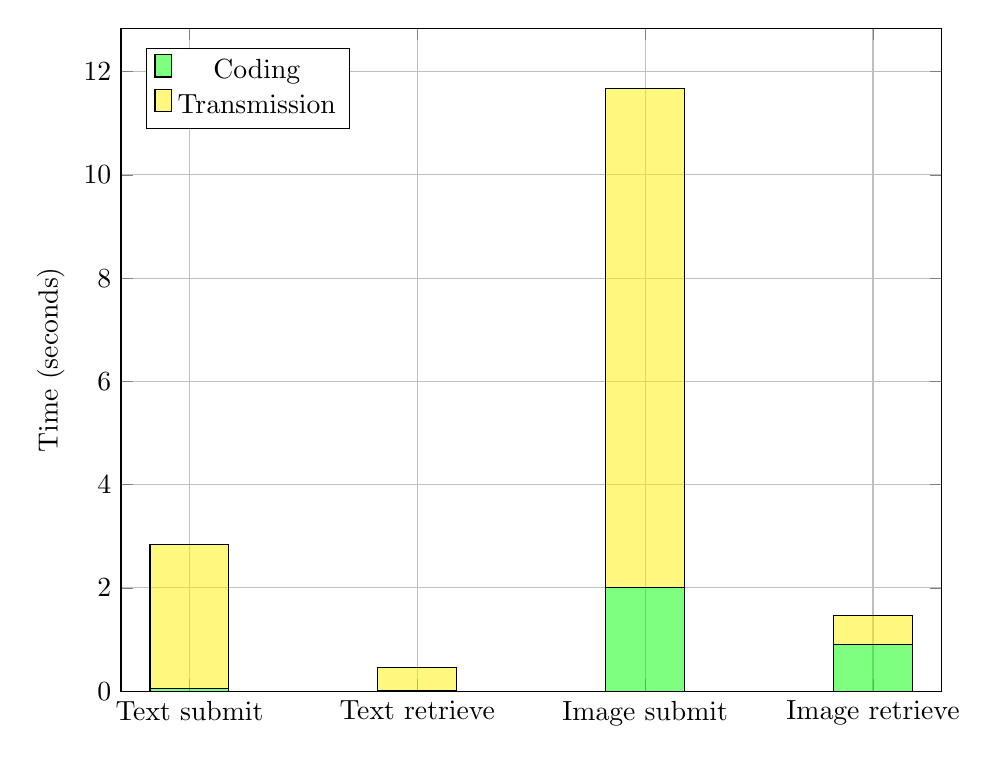
\begin{tikzpicture}
\begin{axis}[grid=major,ybar stacked, 
    symbolic x coords={Text submit,Text retrieve, Image submit, Image retrieve},
    xtick=data,ylabel=Time (seconds), width=12cm, height=10cm,
    legend style={legend pos=north west, area legend},
    bar width=1cm, ymin=0]

    \addplot[fill=green, fill opacity=0.5] coordinates
    {(Text submit,0.0444) (Text retrieve,0.0172) (Image submit,2.0074) (Image retrieve,0.9044)};
    
    \addplot[fill=yellow, fill opacity=0.5] coordinates
    {(Text submit,2.8013) (Text retrieve,0.4446) (Image submit,9.6655) (Image retrieve,0.5662)};
    
    \legend{Coding,Transmission}

\end{axis}
\end{tikzpicture}
    \caption{Average timing results for a 10,000 chracter note and an (approximately) 50 KiB image.}
    \label{graph:txt-sync}
  \end{center}
\end{figure}


\begin{figure}[tbph]
    \begin{center}
\begin{tikzpicture}
\begin{axis}[xlabel=Time (seconds), ylabel=Frequency,
grid=major,const plot, ymin=0, enlargelimits=false,
width=12cm, height=5cm, legend style={area legend}]

    \addplot[fill=blue, fill opacity=0.5] table[x=t,y=Text] {gfx/async_text_hist.data};
    
    \addplot[fill=red, fill opacity=0.5] table[x=t,y=Text_c] {gfx/async_text_hist.data};
    
    \addplot+[sharp plot,blue, mark=no marker] coordinates
        {(6.403,0) (6.403,56)};
        
    \addplot+[sharp plot,red, mark=no marker] coordinates
        {(3.463,0) (3.463,56)};
    
    \legend{Cache off,Cache on}
\end{axis}
\end{tikzpicture}
    \caption{Histogram of 400 page loading times for a newsfeed containing 15 encrypted messages}
    \label{graph:txt-hist}
  \end{center}
\end{figure}

\begin{figure}[tbph]
    \begin{center}
\begin{tikzpicture}
\begin{axis}[xlabel=Time (seconds), ylabel=Frequency,
grid=major,const plot, ymin=0, enlargelimits=false,
width=12cm, height=5cm, legend style={area legend}]
    
    \addplot[fill=blue, fill opacity=0.5] table[x=t,y=Images] {gfx/async_image_hist.data};
    
    \addplot[fill=red, fill opacity=0.5] table[x=t,y=Images_c] {gfx/async_image_hist.data};
    
    \addplot+[sharp plot,blue, mark=no marker] coordinates
        {(19.169,0) (19.169,130)};

    \addplot+[sharp plot,red, mark=no marker] coordinates
        {(4.067,0) (4.067,130)};
    
    \legend{Cache off,Cache on}
    
\end{axis}
\end{tikzpicture}
    \caption{Histogram of 400 page loading times for a newsfeed containing 15 encrypted images}
    \label{graph:img-hist}
  \end{center}
\end{figure}


\begin{figure}[tbph]
    \begin{center}
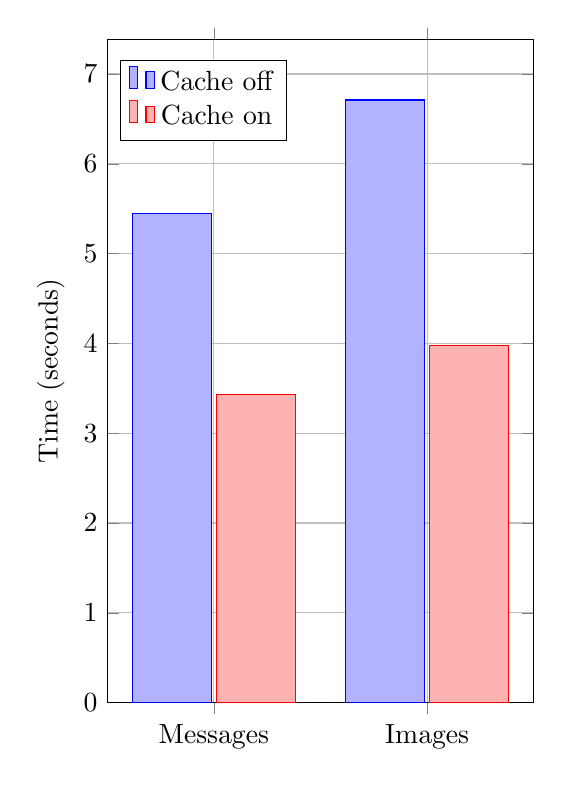
\begin{tikzpicture}
\begin{axis}[grid=major,ybar, 
    symbolic x coords={Messages,Images},
    xtick=data,ylabel=Time (seconds), width=7cm, height=10cm,
    legend style={legend pos=north west, area legend},
    bar width=1cm,enlarge x limits=0.5,ymin=0]

\addplot coordinates { (Messages,5.4457) (Images,6.7105) };
\addplot coordinates { (Messages,3.4306) (Images,3.9765) };
\legend{Cache off, Cache on}

\end{axis}
\end{tikzpicture}
    \caption{Average time before first encrypted item loads.}
    \label{graph:time-first}
  \end{center}
\end{figure}






\begin{figure}
    \begin{center}
    
        \begin{tikzpicture}
        \begin{axis}[grid=major,ycomb,
        ylabel=Time (ms), 
        width=12cm, height=5cm,
        bar width=0.3cm, ymin=0, xmin=2, xmax=15, enlarge x limits=0.04]
        \addplot[blue] table[x=Item,y=Text] {gfx/async.data};
        \end{axis}
        \end{tikzpicture}
    
        \begin{tikzpicture}
        \begin{axis}[grid=major,ycomb,
        ylabel=Time (ms), xlabel=Message,
        width=12cm, height=5cm,
        bar width=0.3cm, ymin=0, xmin=2, xmax=15, enlarge x limits=0.04]
        \addplot[red] table[x=Item,y=Text_c] {gfx/async.data};
        \end{axis}
        \end{tikzpicture}

    \caption{Average time interval between successive message loads, with caching turned off and on (top and bottom respectively).}
    \label{graph:time-rest}
    \end{center}
\end{figure}




\begin{figure}[tbph]
\begin{center}
    
\begin{tikzpicture}
\begin{axis}[grid=major,ycomb,
ylabel=Time (ms), 
width=12cm, height=5cm,
bar width=0.3cm, ymin=0, xmin=2, xmax=15, enlarge x limits=0.04]

\addplot[blue] table[x=Item,y=Image] {gfx/async.data};

\end{axis}
\end{tikzpicture}

\begin{tikzpicture}
\begin{axis}[grid=major,ycomb,
ylabel=Time (ms),xlabel=Image,
width=12cm, height=5cm,
bar width=0.3cm, ymin=0, xmin=2, xmax=15, enlarge x limits=0.04]

\addplot[red,] table[x=Item,y=Image_c] {gfx/async.data};

\end{axis}
\end{tikzpicture}

\caption{Average time interval between successive image loads, with caching turned off and on (top and bottom respectively).}
\label{graph:time-rest}
\end{center}
\end{figure}




\begin{itemize}
    \item Automated results. Mean times for submit and retrive, highlight what portion spent processing and what spent waiting for rest i.e. waiting for HTTP requests to come back.
    \item 
\end{itemize}